%%%%%%%%%%%%%%%%%%%%%%%%%%%%%%%%%%%%%%%%%
% Journal Article
% LaTeX Template
% Version 1.3 (9/9/13)
%
% This template has been downloaded from:
% http://www.LaTeXTemplates.com
%
% Original author:
% Frits Wenneker (http://www.howtotex.com)
%
% License:
% CC BY-NC-SA 3.0 (http://creativecommons.org/licenses/by-nc-sa/3.0/)
%
%%%%%%%%%%%%%%%%%%%%%%%%%%%%%%%%%%%%%%%%%

%----------------------------------------------------------------------------------------
%	PACKAGES AND OTHER DOCUMENT CONFIGURATIONS
%----------------------------------------------------------------------------------------

\documentclass{article}

%\documentclass{aastex}  % version 5.0 or prior
%\usepackage{natbib}



\usepackage{graphicx}
\usepackage{lipsum} % Package to generate dummy text throughout this template
%\usepackage[sc]{mathpazo} % Use the Palatino font
\usepackage[T1]{fontenc} % Use 8-bit encoding that has 256 glyphs
\linespread{1.05} % Line spacing - Palatino needs more space between lines
\usepackage{microtype} % Slightly tweak font spacing for aesthetics

\usepackage[margin=1in,columnsep=20pt]{geometry} % Document margins
\usepackage{multicol} % Used for the two-column layout of the document
\usepackage[hang, small,labelfont=bf,up,textfont=it,up]{caption} % Custom captions under/above floats in tables or figures
\usepackage{booktabs} % Horizontal rules in tables
\usepackage{float} % Required for tables and figures in the multi-column environment - they need to be placed in specific locations with the [H] (e.g. \begin{table}[H])
\usepackage{hyperref} % For hyperlinks in the PDF
\usepackage{subcaption}

\usepackage{lettrine} % The lettrine is the first enlarged letter at the beginning of the text
\usepackage{paralist} % Used for the compactitem environment which makes bullet points with less space between them
\usepackage{amsmath}
\usepackage{abstract} % Allows abstract customization
\renewcommand{\abstractnamefont}{\normalfont\bfseries} % Set the "Abstract" text to bold
\renewcommand{\abstracttextfont}{\normalfont\small\itshape} % Set the abstract itself to small italic text

\usepackage{titlesec} % Allows customization of titles
%\renewcommand\thesection{\Roman{section}} % Roman numerals for the sections
%\renewcommand\thesubsection{\Roman{subsection}} % Roman numerals for subsections
%\renewcommand\thesubsubsection{\Alph{subsubsection}} % Roman numerals for subsections
\titleformat{\section}[block]{\LARGE\scshape}{\thesection}{1em}{} % Change the look of the section titles
\titleformat{\subsection}[block]{\Large\scshape}{\thesubsection}{1em}{} % Change the look of the section titles
\titleformat{\subsubsection}[block]{\large\scshape}{\thesubsubsection}{1em}{} % Change the look of the section titles

\usepackage{fancyhdr} % Headers and footers
\pagestyle{fancy} % All pages have headers and footers
\fancyhead{} % Blank out the default header
\fancyfoot{} % Blank out the default footer
\fancyhead[C]{Montana State University \quad $\bullet$ \quad CSCI 466 Artificial Intelligence \quad $\bullet$ \quad Group 21} % Custom header text
\fancyfoot[RO,LE]{\thepage} % Custom footer text

\newcommand{\ve}[1]{\boldsymbol{\mathbf{#1}}}

\title{\vspace{-15mm}\fontsize{24pt}{10pt}\selectfont\textbf{CSCI 446 Artificial Intelligence \\[2mm] Project 4 Design Report} } % Article title
\date{\today}
\author{
\large
\textsc{Roy Smart} \and \textsc{Nevin Leh} \and \textsc{Brian Marsh}\\[2mm] % Your name
}


%----------------------------------------------------------------------------------------

\begin{document}

	\maketitle % Insert title
	\thispagestyle{fancy} % All pages have headers and footers
	\normalsize

	\section{Introduction}
		Within the field of machine learning, there is a type of unsupervised learning known as reinforcement learning.  An agent using reinforcement learning makes actions in its environment and observes the rewards that it obtains from such actions.  Using many observations of the environment, the agent may be trained to maximize its cumulative rewards through the problem that it attempts to solve.
	\section{The Racetrack Problem}
		Using reinforcement learning, we will attempt to solve the racetrack problem.  The goal of this problem is simply to control the movement of a race car as it moves along a track.  Performance is based upon the number of time steps that the car requires to reach the finish.  If the car moves into a wall, a penalty will be applied, thus decreasing performance.  The car is represented by four variables at any given state: $x(t)$ and $y(t)$ (horizontal and vertical components of the car's location at time $t$) and $\dot{x}(t)$ and $\dot{y}(t)$ (horizontal and vertical components of the car's velocity at time $t$).  Control of the car can only be achieved by manipulating the velocity of the car, using the variables $a_x$ and $a_y$ (horizontal and vertical components of the acceleration vector).  The problem is complicated by the addition of a 20\% chance of failure for any acceleration action.  Additionally, the agent will be tested on multiple tracks of varying shape.
	\section{Reinforcement Learning Algorithms}
		\subsection{Value Iteration}
	\section{Q-Learning}
		\subsection{Description}
			\textit{Q-learning} is a model-free reinforcement learning method for determining optimal action-selection policies \cite{ai}. An agent using this method leverages a quantity known as the $Q$-value to derive the optimal action $a$ for each state $s$. The $Q$-value, $Q(s,a)$ describes the expected utility for every action in every state within the environment and is learned by the agent using temporal difference learning.
			An expression to calculate the $Q$-value is given by \cite{ai} as
			\begin{equation}
				Q(s,a) \leftarrow Q(s,a) + \alpha \left[ R(s) + \gamma \max_{a'} Q(s',a') - Q(s,a) \right]
				\label{ql}
			\end{equation}
			where $a$ is the action that was executed in state $s$ that resulted in state $s'$ and $R(s)$ is the reward function. The constants $\alpha$ and $\gamma$ are known respectively as the learning rate and the discount factor. Equation \ref{ql} is used as an update rule to adjust the value of $Q(s,a)$ for each action-state pair in every time trial undertaken by the agent. Using this simple update rule and randomly initialized $Q$-values for every action-state, an agent can learn how to navigate an environment.
		\subsection{Design Implications}
			In the racetrack problem $Q$-Learning will need to learn the $Q$-value for all nine acceleration options for every possible velocity vector at every possible position vector.
			Since the racetracks are reasonably small, we can afford to sore the table of $Q$-values in memory. We will base our $Q$-learning agent off of the function \textsc{Q-Learning-Agent} provided in Figure 21.8 of \cite{ai}. To ease the training time, we will incrementally train the $Q$-learning agent by beginning training close to the finish line, and then increasing the distance as the agent learns each section.
	\section{Software Design}
	For this project we will be using an environment and agent model similar to the wumpus world. Instead of a board we will have a \texttt{Track} class that reads in the different tracks from a text file. To run the experiments we will have an \texttt{Environment Engine} for each \texttt{Track} and \texttt{Agent} combo. 
	
	The \texttt{Agent} will be a virtual class that contains data such as the max acceleration values. It will also contain the virtual method \texttt{learn}. Each concrete class will be the implementation of our reinforcement learners. Each of these classes will contain an overridden learn method and algorithm specific functionality. The key difference between the wumpus world \texttt{Agent} and this \texttt{Agent} is the fact that in this case the \texttt{Agent} can see the whole board from the start.
	\begin{figure}[h!]
		\centering
		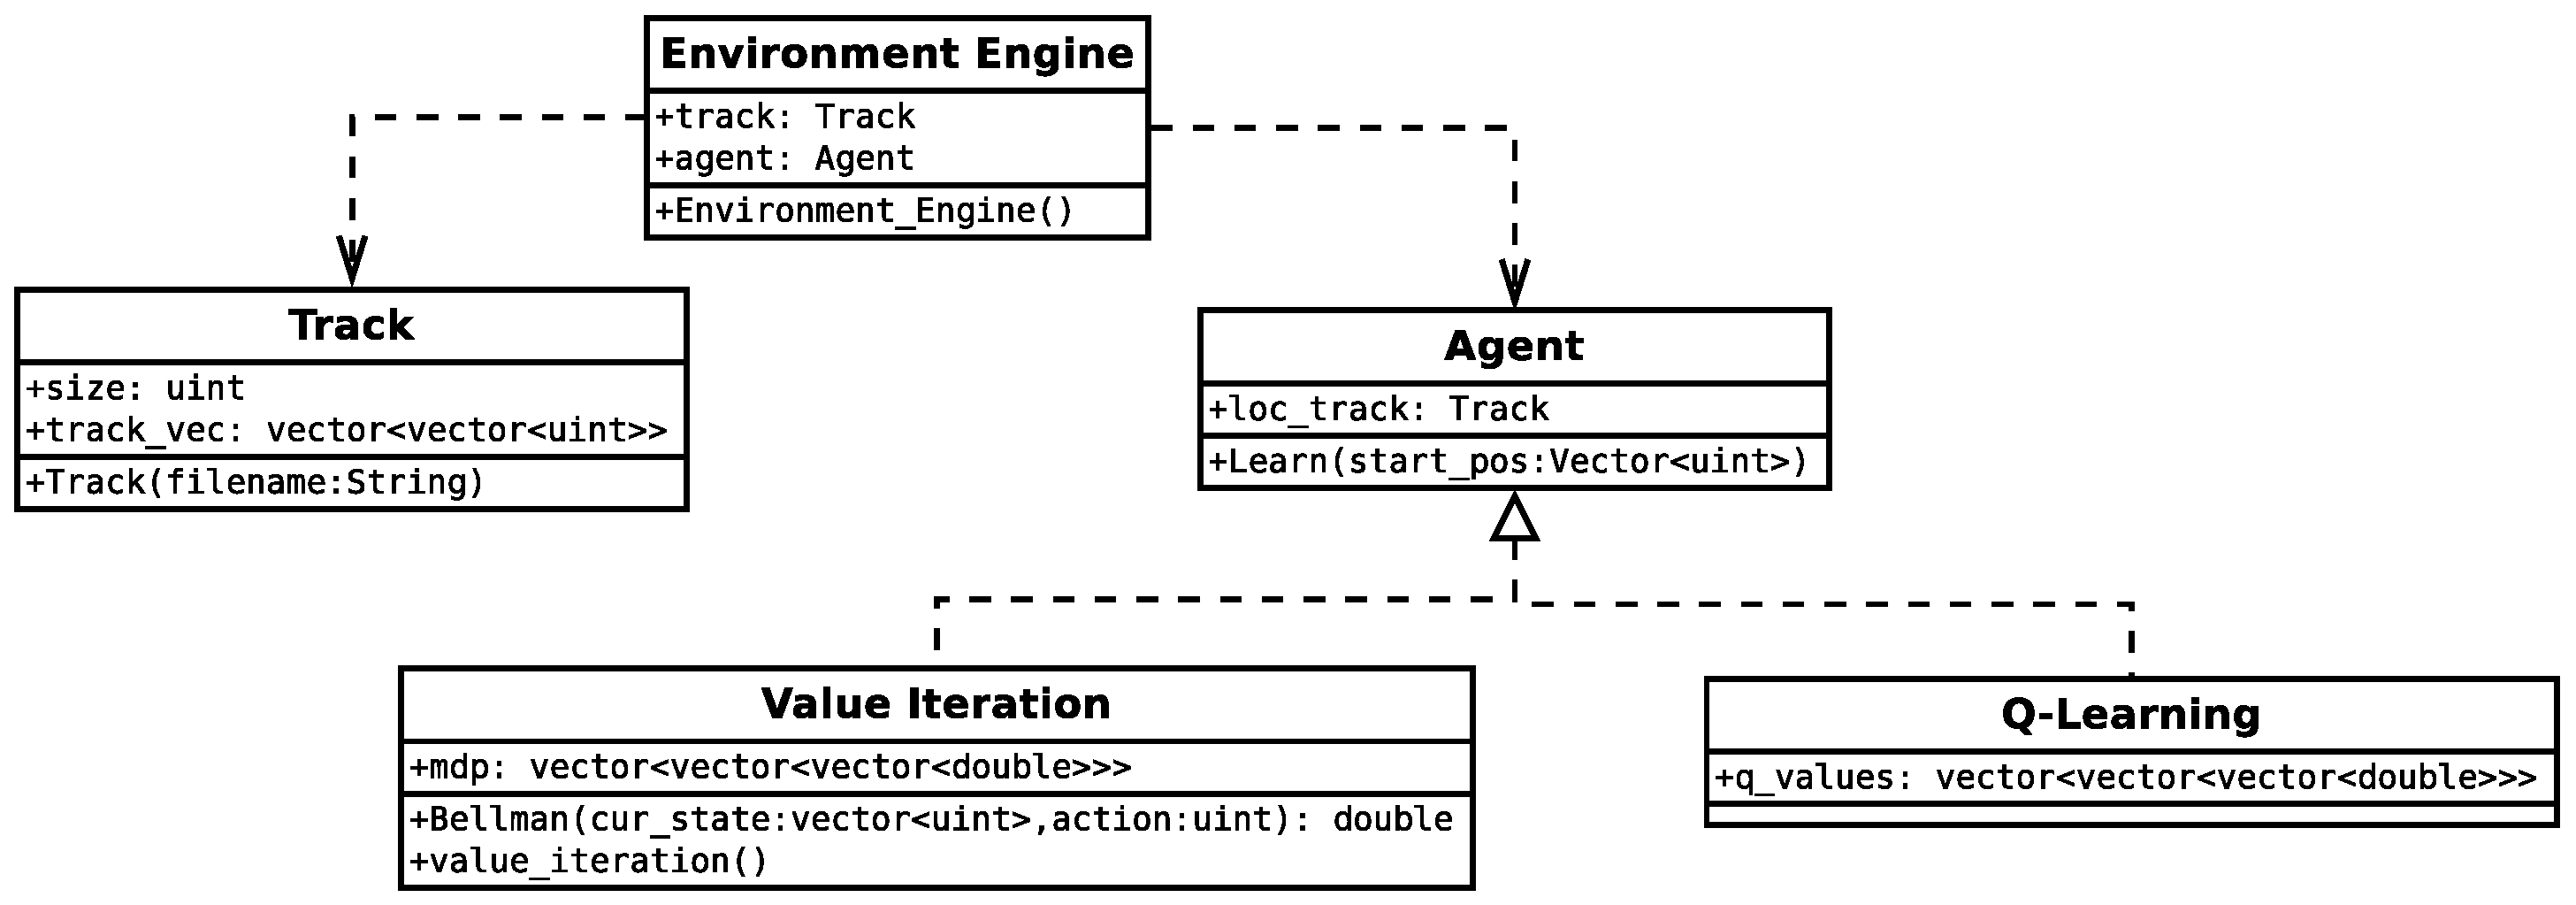
\includegraphics[width=0.99\textwidth]{Diagrams/uml}
		\caption{UML of our design}
	\end{figure}
	\section{Experiment Design}
		 For each agent we will generate learning curves that describe the number of steps required to reach the goal state vs. the number of training iterations. We will also track the number of times each agent runs into a wall and needs to be restarted. Each agent will be trained at least 10 times to determine reliable learning curves.
	\section{Summary}

	%\bibliographystyle{apj}
	\bibliographystyle{apalike}	
	\bibliography{sources}
\end{document}
